\section{Computerarithmetik}

\subsection{Ganzzahlig}
\begin{tabular}{|p{3cm}|p{4.5cm}|p{4.5cm}|p{4.5cm}|}
	\hline
	Darstellung & Sign Magnitude & 1er Komplement & 2er Komplement\\
	\hline
	Zahlenbereich & $-(2^{n-1}-1)$ bis $+(2^{n-1}-1)$ & $-(2^{n-1}-1)$ bis +$(2^{n-1}-1)$ & $-2^{n-1}$ bis +$(2^{n-1}-1)$\\
	\hline
	Vorteil & Vorzeichen kann einfach durch Vorzeichenbit festgestellt werden. & Vorzeichen kann einfach durch MSB festgestellt werden. Addition und Subtraktion einfach realisierbar. & Vorzeichen kann einfach durch MSB festgestellt werden. Addition und Subtratkion einfach realisierbar \\ 
	\hline
	Nachteil & Positive und negative Null. Addition/Subtraktion kompliziert. & Positive und negative Null. & Bereich nicht ganz symmetrisch\\
	\hline
	Beispiel +5 & 0101 & 0101 & 0101 \\
	Beispiel -5 & 1101 & 1010 & 1011 \\
	\hline
\end{tabular}

\subsubsection{Addition/Subtraktion}
Wird direkt mit der Arithmetic Logic Unit (ALU) durchgeführt.

\subsubsection{Multiplikation}
\paragraph {Multiplikation mit Zweierpotenzen}
Die Multiplikation mit Zweierpotenzen ist ein Spezialfall, der sehr effizient umgesetzt werden kann. Die Multiplikation einer Zahl $x$ mit $2^n$ entspricht einem Schieben der Zahl $x$ um $n$ Stellen nach links.

\paragraph{Allgemeine Multiplikation}
\begin{multicols}{2}
	Implementation algorithmisch: Langsam, wenig Aufwand
	\begin{itemize}
		\item Mikroprogramm
		\item Softwareemulation
	\end{itemize}
	Implementation Hardware: Schnell, viel Aufwand
	\begin{itemize}
		\item In vielen uC's drin, vor allem RISC (MSP430)
		\item Im DSP ist HW-Multiplizierer ein Muss
	\end{itemize}
	\columnbreak
	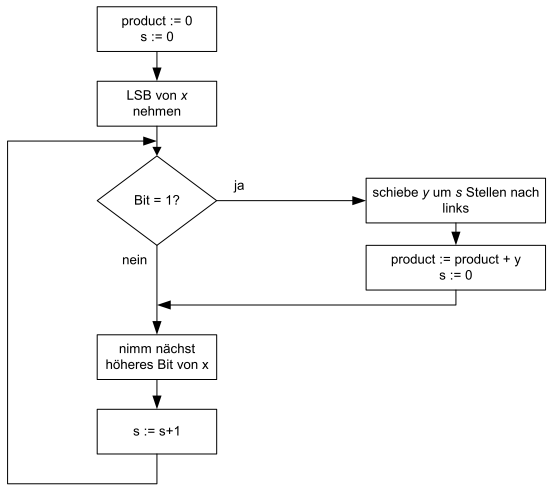
\includegraphics[width=0.3\textwidth]{images/Arithmetik/Ganzzahlig_Multiplikation}
\end{multicols}

\subsubsection{Division}
\paragraph {Division mit Zweierpotenzen}
Die Division durch Zweierpotenzen ist ein Spezialfall, der sehr effizient umgesetzt werden kann. Die Division einer Zahl $x$ durch $2^n$ entspricht einem Schieben der Zahl $x$ um $n$ Stellen nach rechts.

\paragraph {Allgemeine Division}
Implementation algorithmisch: Langsam, wenig Aufwand
\begin{itemize}
	\item Mikroprogramm
	\item Softwareemulation
\end{itemize}
Implementation Hardware: Schnell, viel Aufwand
\begin{itemize}
	\item In vielen uC's drin, vor allem RISC (MSP430)
	\item da die Division die seltenste Operation ist, wird speziell bei Microcontrollern nur selten ein Hardware-Dividierer verwendet
\end{itemize}

\subsubsection{Skalierung}
\begin{itemize}
	\item Aus Effizienzgründen wird insbesondere bei Mikrocontrollern versucht, so viel wie möglich mit Integer-Arithmetik zu lösen
	\item Quantisierung auf 1 Bit kann bei kleinen Werten zu Ungenauigkeiten führen
	\item Lösung: durch Skalierung soll Dynamikbereich, d.h. der Wertebereich der ganzen Zahl, möglichst ausgenutzt werden
	\item Skalierungen mit Zweierpotenzen sind viel effizienter als solche mit Dezimalzahlen
	\item Wenn möglich immer mit Zweierpotenzen skalieren	
\end{itemize}

\subsection{Arithmetische Schaltungen}
\subsubsection{Addierer}
Wichtigste arithmetische Funktion, n-Addierer werden auf 1-Bit Addierer zurück geführt.
\paragraph{1 Bit Halbaddierer:}
\begin{minipage}{0.5\textwidth}
	\centering
	\begin{tabular}{|c | c | c | c |}
		\hline
		A & B & Sum & Carry\\
		\hline
		0 & 0 & 0 & 0\\
		\hline
		0 & 1 & 1 & 0\\
		\hline
		1 & 0 & 1 & 0\\
		\hline
		1 & 1 & 0 & 1\\
		\hline
	\end{tabular}
\end{minipage}
\begin{minipage}{0.9\textwidth}
	\centering
	\begin{flushleft}
		{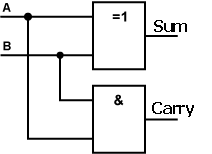
\includegraphics[width=0.3\textwidth]{images/Arithmetik/halbaddierer.png}}
	\end{flushleft}
\end{minipage}\\ \\

\paragraph{1 Bit Volladierer:}
\begin{minipage}{0.35\textwidth}
	\begin{tabular}{|c | c | c | c | c |}
		\hline
		A & B & Carry In & Sum & Carry Out\\
		\hline
		0 & 0 & 0 & 0 & 0\\
		\hline
		0 & 0 & 1 & 1 & 0\\
		\hline
		0 & 1 & 0 & 1 & 0\\
		\hline
		0 & 1 & 1 & 0 & 1\\
		\hline
		1 & 0 & 0 & 1 & 0\\
		\hline
		1 & 0 & 1 & 0 & 1\\
		\hline
		1 & 1 & 0 & 0 & 1\\
		\hline
		1 & 1 & 1 & 1 & 1\\
		\hline
	\end{tabular}
\end{minipage}
\begin{minipage}{0.9\textwidth}
	\begin{flushleft}
		{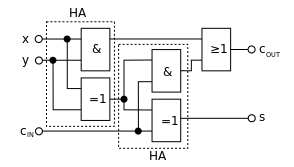
\includegraphics[width=0.7\textwidth]{images/Arithmetik/volladdierer.png}}
	\end{flushleft}
\end{minipage}

\paragraph {Ripple Carry Adder (4 Bit)}
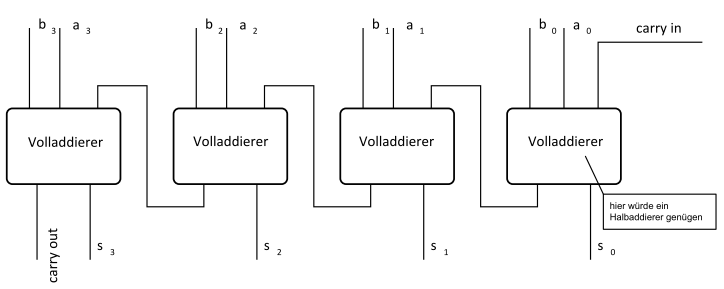
\includegraphics[width=1\textwidth]{images/Arithmetik/Ripple_Carry_Adder}
Das niederwertige Carry-Bit wird immer an die nächst höhere Position weitergereicht. Dadurch dauert es eine gewisse Zeit, bis das MSB korrekt ist. Für hohe Wortbreiten zu langsam.

\paragraph{Carry Select Adder}
\begin{itemize}
	\item Obere Worthälfte wird zweimal berechnet 
	\begin{itemize}
		\item einmal für Carry-In = 0 
		\item einmal für Carry-In = 1
	\end{itemize}
	\item Die untere Worthälfte und die beiden oberen Worthälften werden gleichzeitig berechnet.
	\item Das richtige Resultat der oberen Worthälfte wird ausgewählt sobald das Carry der unteren Worthälfte feststeht.
	\item Bei einem $n$ Bit breiten Adder wird idealerweise in $\sqrt{n}$ breite Blöcke aufgeteilt 
	\item Die Ausführungszeit steigt dann nicht linear, sondern nur mit $\sqrt{n}$
	\item Kosten: Erhöhter Hardwareaufwand
\end{itemize}

\paragraph{Carry Look-Ahead Adder}
	\begin{multicols}{2}
		\begin{itemize}
		\item Carrymuss bei jeder Bitposition $i$ entweder fortgepflanzt (propagate, $p_i$) oder generiert (generate, $g_i$) werden. 
		\item  $p_i$ und $g_i$ sind nur von den Eingängen $a_i$ und $b_i$ abhängig, nicht aber von den Carries der vorherigen Stufen. 
		\begin{equation}
			p_i = a_i \oplus b_i \newline	
		\end{equation}
		\begin{equation}
		g_i = a_i * b_1		
		\end{equation}
		\begin{equation}
		c_{i+1} = g_i + p_i * c_i		
		\end{equation}
		\item  Jedes einzelne Carry kann somit als zweistufige Logik von verschiedenen $p_i$ und $g_i$ implementiert werden. 
	\end{itemize}	
\columnbreak			
	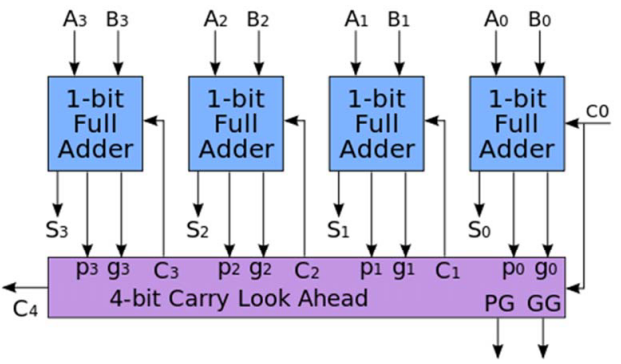
\includegraphics[width=0.5\textwidth]{images/Arithmetik/Carry_Look_Ahead_Adder}
\end{multicols}

\subsubsection{Subtrahierer}
\begin{equation}
A-B = A + (-B)	
\end{equation}
\begin{itemize}
	\item Subtraktion wird zurückgeführt auf Addition
	\item (-B) kann gebildet werden, indem alle Bits von B invertiert werden und 1 addiert wird.
	\item 1 addieren erfolgt durch Anlegen einer '1' bei $Carry_0$
	\item Damit der Addierer mit minimalem Zusatzaufwand auch als Subtrahierer verwendet werden kann, wird deshalb auch an der Bitposition 0 ein Volladdierer eingesetzt
\end{itemize}

\subsubsection{Schiebeeinheit (Shifter)}
\begin{itemize}
	\item Ein Shifter kann mit einem Schieberegister implementiert werden
	\item Der Nachteil dabei ist, dass pro Clockzyklus nur um ein Bit nach links oder rechts geschoben werden kann. Zudem ist das Schieberegister eine sequentielle Schaltung und benötigt Flip Flops.
	\item Oft muss um eine beliebige Anzahl Stellen möglichst  in einem Schritt geschoben werden
	\item Schieben kann auch mittels einer kombinatorischen Schaltung erreicht werden 
	\item In der Praxis wird meist ein Barrel Shifter eingesetzt. Dieser kann innerhalb eines Zyklus um eine beliebige Anzahl Stellen schieben. Der Barrel Shifter ist rein kombinatorisch.	
\end{itemize}

\begin{multicols}{2}
	\paragraph{Kombinatorischer 8 Bit Shifter nach links (C=0) bzw. rechts (C=1)}
	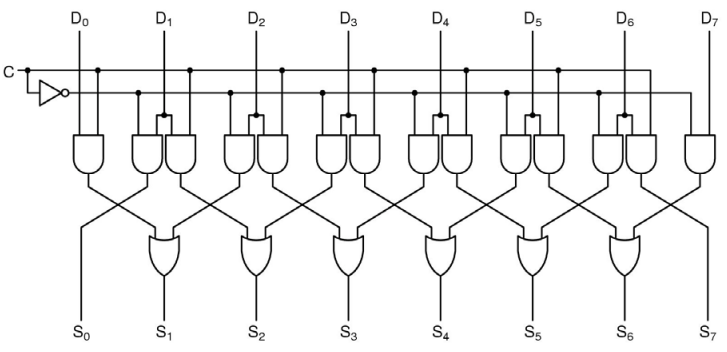
\includegraphics[width=0.3\textwidth]{images/Arithmetik/Shifter_1}

	\paragraph{4 Bit Crossbar Barrel Shifter}
	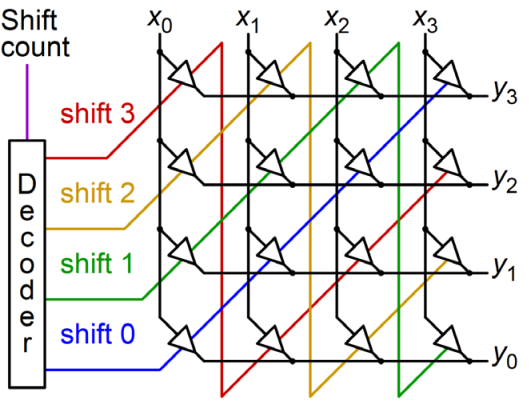
\includegraphics[width=0.2\textwidth]{images/Arithmetik/Shifter_2}
\end{multicols}

\subsubsection{Sättigungsarithmetik}
\begin{itemize}
	\item Besonders bei DSPs wird die Sättigungsarithmetik als Option eingesetzt 
	\item Wenn der maximal darstellbare Wert inkrementiert werden soll, ergibt das nicht einen Overflow sondern der Wert bleibt auf seinem Maximalwert 
	\item Analog wird der minimale Wert behandelt: bei signedTypen verbleibt der minimale negative Wert, bei unsignedTypen der Wert Null
\end{itemize}

\subsection{Fixpunkt (Fixed Point)}
\begin{itemize}
	\item Die Hardware für Fixed Point Arithmetic ist einfacher als die Floating Point Arithmetic, d.h. sie kann einfacher implementiert werden
	\item Wie der Name sagt, sitzt der Dezimalpunkt an einer fixen Stelle. Die Stellen rechts vom Dezimalpunkt werden als negative Zweierpotenzen interpretiert
	\item  Für Fixed Point-Berechnungen kann die Integereinheit verwendet werden
	\item Eigentlich erhält das LSB einfach nicht mehr den Wert 1, sondern beispielsweise den Wert $2^{-6}$, d.h $\frac{1}{64} = 0.015625$
	\item  Davon ausgehend kann mit der Integereinheitganz normal gerechnet werden. 
	Fixed Point Berechnungen sind deshalb sehr effizient
\end{itemize}

\subsection{Gleitkomma (Floating Point)}
\begin{multicols}{2}
	\begin{equation}
	(-1)^S\cdot M \cdot B^E
	\end{equation}
	S = Vorzeichen (float: 1 bit double:1 bit)\\
	M = Mantisse (float:23 bit double: 52 bit)\\
	B = Basis \\
	E = Exponent (float:8 bit double:11 bit)\\
\columnbreak
	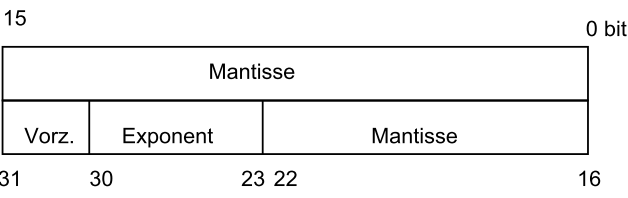
\includegraphics[width=0.5\textwidth]{images/Arithmetik/floating_point}
\end{multicols}

\subsubsection{Floating Point Unit (FPU)}
\begin{itemize}
	\item Eine FPU ist eine Hardwareimplementation für die Berechnung von Floating Point Zahlen
	\item Eine FPU-Implementation rechnet die FP-Operationen mindestens eine Grössenordnung schneller als Softwareimplementationen
	\item Nebst den Grundrechenarten rechnet die FPU auch Wurzeln, teilweise auch trigonometrische Funktionen, etc.
\end{itemize}

\subsubsection{Addition}
\begin{enumerate}
	\item Die beiden Exponenten subtrahieren, um festzustellen, welcher der grössere ist. Der grössere Exponent wird als resultierender Exponent verwendet. Die Mantisse der kleineren Zahl muss zudem vor der Addition um diesen Differenzbetrag verschoben werden. 
	\item Die Mantisse der kleineren Zahl verschieben und zur grösseren addieren. 
	\item Die Mantisse wieder normalisieren, d.h. für die Mantisse M muss immer gelten: $1 \leq M \leq 2$. Dies bedingt unter Umständen auch eine Anpassung des Exponenten.	
\end{enumerate}
Für einen Floating Point Adder werden mindestens folgende Elemente benötigt: Integer-Addierer/Subtrahierer, Komparatoren und Schiebeeinheiten (Shifter)

\subsubsection{Subtraktion}
Der Floating Point Subtrahierer kann analog zum Addierer implementiert werden.

\subsubsection{Multiplikation}
\begin{equation}
	m_1 \cdot B^{e1} \cdot m_2 \cdot B^{e2} = m_1 \cdot m_2 \cdot B^{e1 + e2}
\end{equation}
\begin{enumerate}
	\item Die beiden Exponenten müssen addiert werden 
	\item Die beiden Mantissen müssen multipliziert werden 
	\item Die Mantisse wieder normalisieren, d.h. für die Mantisse M muss immer gelten: $1 \leq M \leq 2$. Dies bedingt unter Umständen auch eine Anpassung des Exponenten.	
\end{enumerate}
Für einen Floating Point Multiplier werden mindestens folgende Elemente benötigt: Integer-Addierer/Subtrahierer, Integer-Multiplizierer und Schiebeeinheiten (Shifter)

\subsubsection{Division}
\begin{equation}
\frac{m_1 \cdot B^{e1}}{m_2 \cdot B^{e2}} = \frac{m_1}{m_2} \cdot B^{e1 - e2}
\end{equation}
\begin{enumerate}
	\item Die beiden Exponenten müssen subtrahiert werden 
	\item  Die beiden Mantissen müssen dividiert werden 
	\item Die Mantisse wieder normalisieren, d.h. für die Mantisse M muss immer gelten: $1 \leq M \leq 2$. Dies bedingt unter Umständen auch eine Anpassung des Exponenten.	
\end{enumerate}
Für einen Floating Point Divider werden mindestens folgende Elemente benötigt: Integer-Addierer/Subtrahierer, Integer-Dividierer und Schiebeeinheiten (Shifter) \\
Die Floating Point Division ist relativ selten (ca. 5\% der Grundrechenarten im Normalfall). Aus diesem Grund wird oft kein Hardware-Dividierer angeboten. Häufig wird eine Multiplikation mit der Reziproken gerechnet. Die Reziproke kann nur mit Additionen und Multiplikationen gerechnet werden
\begin{equation}
\frac{x}{y} = \frac{1}{y} \cdot x
\end{equation}

\subsubsection{Berechnung von beliebigen Kurvenverläufen}
\begin{itemize}
	\item Der Verlauf von beliebigen Kurven wird häufig in Lookup Tables gespeichert
	\item Für Werte zwischen zwei Stützwerten wird interpoliert, normalerweise linear
	\item Die Genauigkeit nimmt offensichtlich zu, je mehr und je genauere Stützwerte gespeichert werden
	\item Denkbar sind auch Approximationen, wobei nur mit Additionen, Subtraktionen und Multiplikationen gearbeitet werden darf	
\end{itemize}

\subsubsection{Newton-Raphson}
Um eine unäre Funktion wie $sin(x)$ zu berechnen, kann man die Taylorreihe verwenden $sin(x) = x - \frac{x^3}{3!} + \frac{x^5}{5!} - \frac{x^7}{7!}\cdots$ Die Koeffizienten könnten gespeichert werden, jedoch ist die Konvergenz trotz dieser Vereinfachung langsam. 
Eine Methode, welche schneller konvergiert ist das Newton-Raphson Verfahren: 
\begin{equation}
y_{k+1} = y_k - \frac{f(y_k)}{\frac{\partial}{\partial y}f(y_k)}
\end{equation}
Zur Berechnung einer Reziproken $g(x)=\frac{1}{x}=y$ ergibt sich folgende Formel: 
\begin{equation}
y_{k+1} = y_k\cdot (2-x\cdot y_k)
\end{equation}
Wobei $x$ die Zahl aus dem Reziprokwert ist und $y_k$ ein vernünftiger Anfangswert ist. \\

Somit kann auch die Quadratwurzel berechnet werden und zwar via: $\frac{1}{\sqrt{x}} \cdot x = \sqrt{x}$\\
Wobei der Bruch $\frac{1}{\sqrt{x}}$ wie folgt berechnet werden kann:
\begin{equation}
y_{k+1} = 0.5y_k\cdot (3-x\cdot y_k^2)
\end{equation}
Das Newton Verfahren konvergiert quadratisch, d.h mit jedem Durchlauf kann die Genauigkeit verdoppelt werden.

\begin{multicols}{2}
	\paragraph{Herleitung $\frac{1}{x}$}
	\begin{equation}
	g(x)=\frac{1}{x} \equiv y \rightarrow x=\frac{1}{y}
	\end{equation}
	\begin{equation}
	f(y) \equiv \frac{1}{y}-x = 0
	\end{equation}
	\begin{equation}
	\frac{\partial}{\partial y} f(y)=-y^{-2}=-\frac{1}{y^2}
	\end{equation}
	\begin{equation}
	y_{k+1}=y_k-\frac{\frac{1}{y_k}-x}{-\frac{1}{y^2}}
	\end{equation}
	\begin{equation}
	y_{k+1}=y_k \cdot (2-x \cdot y_k)
	\end{equation}
\columnbreak
	\paragraph{Herleitung $\frac{1}{\sqrt{x}}$}
	\begin{equation}
	g(x)=\frac{1}{\sqrt{x}} \equiv y \rightarrow x=\frac{1}{y^2}
	\end{equation}
	\begin{equation}
	f(y) \equiv \frac{1}{y^2}-x = 0
	\end{equation}
	\begin{equation}
	\frac{\partial}{\partial y} f(y)=\frac{-2}{y^3}
	\end{equation}
	\begin{equation}
	y_{k+1}=y_k-\frac{\frac{1}{y_k^2}-x}{\frac{-2}{y^3}}
	\end{equation}
	\begin{equation}
	y_{k+1}=0.5 \cdot y_k \cdot (3-x \cdot y_k^2)
	\end{equation}
\end{multicols}